\section{Languages and Frameworks}

    I have chosen to develop this as a web app as this is the most accessible form of application that can run on any web browser. This also fulfils the requirement of a desktop-scale application [\autoref{requirements-GUI}], maintaining support for variable aspect ratios.

    \subsection{JavaScript}

        \begin{wrapfigure}{r}{0.10\textwidth}
            \centering
            
\includegraphics[width=0.10\textwidth]{js-logo-512.png}
        \end{wrapfigure}

        JavaScript is a web native, interpreted language that runs directly in a browser. It is dynamically typed (which is rectified by the use of TypeScript [\autoref{typescript}]), and has the capability to communicate directly with HTML/CSS environments [\autoref{html/css}]. JavaScript is the most popular framework for web development and is utilised in almost all websites.

        Using JavaScript modules a program can be split into many distinct scripts, allowing for improved project management. In this way JavaScript has the capability to mimic the class structure of Java, a version of the OOP paradigm that I am very familiar with.

    \subsection{TypeScript}
    \label{typescript}

        \begin{wrapfigure}{r}{0.10\textwidth}
            \centering
            
\includegraphics[width=0.10\textwidth]{ts-logo-512.png}
        \end{wrapfigure}

        TypeScript \cite{typescript} is a superset of the JavaScript language, the main difference being that TypeScript has the capabilities for static typing. I have chosen this as it combines the flexible and powerful components of native JavaScript with the clarity, efficiency and maintainability of statically typed languages. Hopefully this will allow me to write code quickly and cleanly, using my IDE's built-in TypeScript development tools.

        TypeScript compiles into native JavaScript code and this is what will be running in the browser when the program is loaded.

        As a quick note, as the static type system for TypeScript was built off of the existing JavaScript system it does include a specific integer type. Instead all numeric values fall under the \mintTS{number} type, therefore in the rest of this document I will refer to variables used as ids or array indices using the \mintTS{number} type as this more accurately reflects the implementation. While its integer status can largely be infered from identifiers or usages.

    \subsection{HTML/CSS}
    \label{html/css}

        The HTML and CSS framework will handle most of the GUI visuals and layout. This will interface directly with my JavaScript object code through DOM-manipulation statements. A few important ones are listed below:

        \begin{itemize}
            \item \mintTS{document.querySelector(<selector>);} To retrieve a reference to the specified element in the document.

            \item \mintTS{element.style.<property>;} Allows access to an elements runtime CSS properties to be edited.

            \item \mintTS{document.createElement(<tag>);} Creates an element with a specified HTML tag that can be subsequently added to the document.

            \item \mintTS{element.appendChild(<childElement>);} Adds the child element as a sub-element of the parent.

            \item \mintTS{element.innerHTML;} Accesses the raw HTML contained within the element as a string to be changed or reassigned.

            \item \mintTS{element.addEventListener(<event>, <callback>);} This will be a vital part of my program, allowing code to respond to document events such as clicks, keypresses and scrolls.
        \end{itemize}

\section{Program overview}

    This program will consist largely of three major components: A road network model; a framework for testing the road model; and a system to handle the display as well as user interaction.

    By the nature of HTML, the front-end of this program will be event based, utilising JavaScript event listeners to respond to user interactions.

    I will be using the model-view-controller design pattern to manage the interactions between these components, the basis of which is summarised in \autoref{model-view-controller}

    \begin{figure}
        \centering
        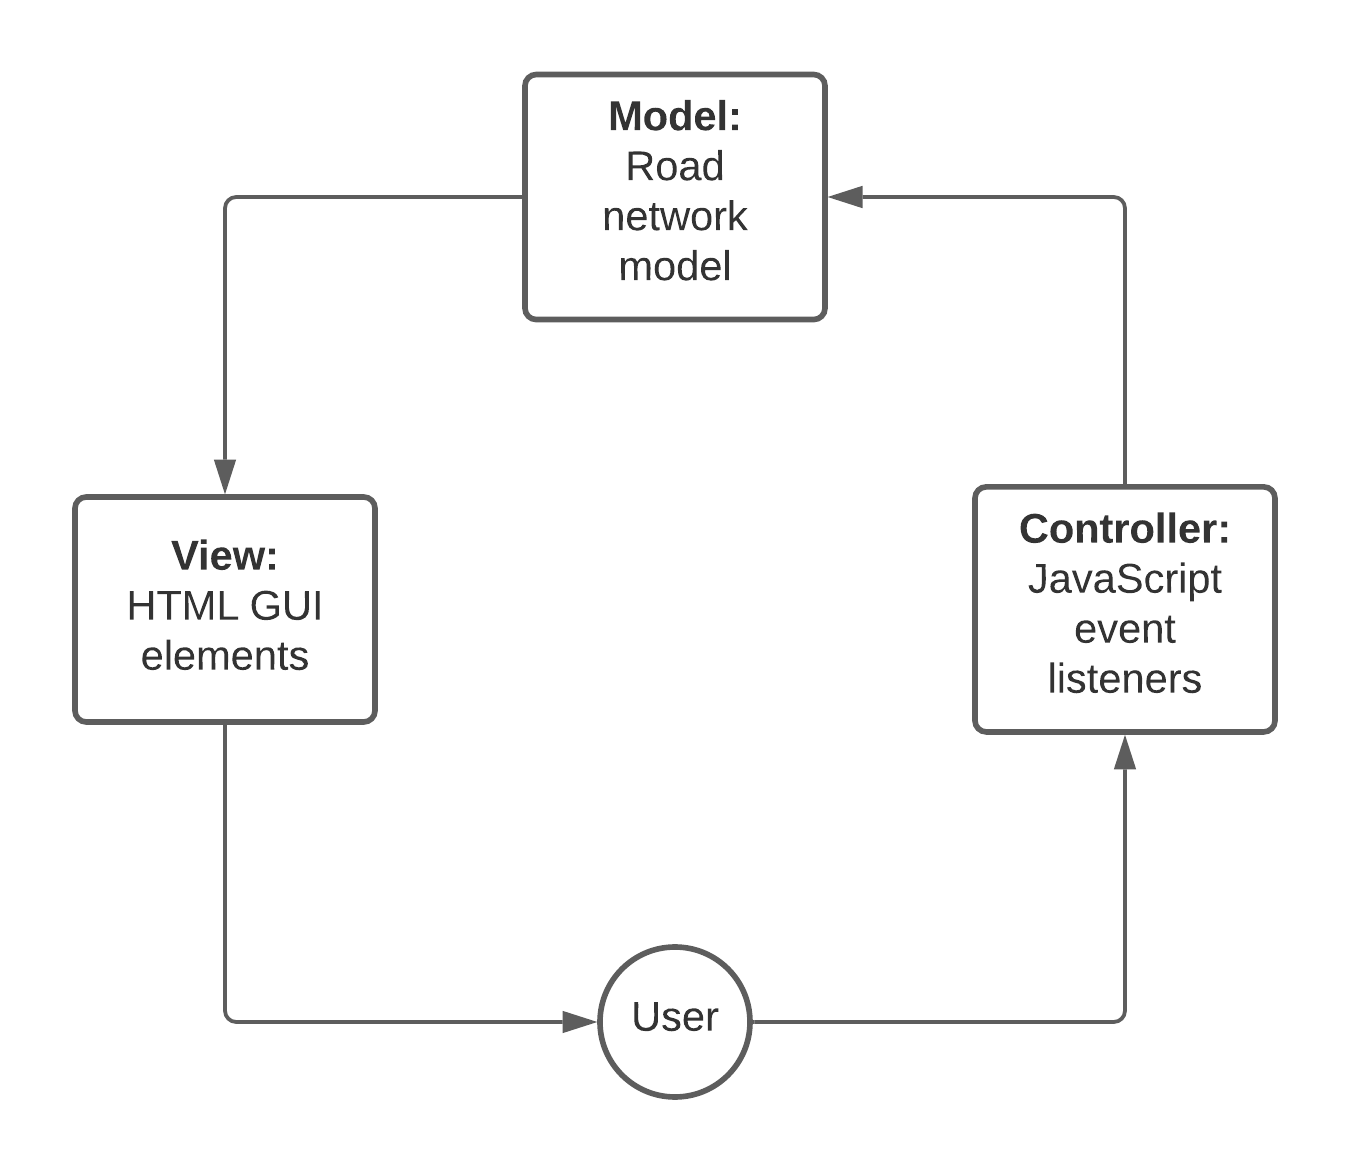
\includegraphics[width=0.5\textwidth]{model-view-controller.png}
        \caption{Model-view-controller design pattern}
        \label{model-view-controller}
    \end{figure}

    Note that in this framework the 'Model' includes both the Road network model and the testing component together, although these will be separately implemented.

\section{Network Builder}

    \subsection{User Interaction}

        As specified in my analysis section, the user input scheme will be based largely off of mouse interactions similar to that of the Mini Motorways computer game [\autoref{mini-motorways}]. The controls are listed in \autoref{user-interaction-specification}:

        \begin{table}
            \centering
            \begin{tabular}{|p{0.45\textwidth}|p{0.45\textwidth}|}
                \hline
                \textbf{Input} & \textbf{Result}\\
                \hline
                Left-click and drag on and empty space & Pan the display along the path of the cursor\\\hline

                Lift-click and drag on an existing vertex & Move the targeted node along the path of the cursor until button is released\\\hline

                Shift-left-click an existing vertex and drag to another existing vertex & Connect an edge between the two targeted vertices\\\hline

                Shift-left-click an existing vertex and drag to an empty space & Create new node at the end point and connect with the existing node\\\hline

                Shift-Left-click on empty space & Create new node at the selected point with no connections\\\hline

                Shift-Left-click on node & Remove the node from the network\\\hline
            \end{tabular}
            \caption{User interactions with graph model}
            \label{user-interaction-specification}
        \end{table}

        \subsubsection{State Machine}

            This behaviour can be modelled by a finite state machine as shown in \autoref{network-builder-state-machine}. This will be implemented using a map that relates the current state and triggered event to a new state and a callback that is called when the transition occurs.

            Since TypeScript \mintTS{Map} types must be keyed by a single immutable object I will need to define a method for converting the state and event into this form. I will represent the possible states of the program and the transtition events as enums, allowing both these values to be represented as natural numbers. Now I can use the Cantor pairing function \cite{cantor-pairing-function} to map each pair of non-negative integers to distinct integers. The pairing function (usually denoted by $\pi$) is defined as: \[\pi(k_1, k_2) := \frac{1}{2}(k_1 + k_2)(k_1 + k_2 + 1) + k_2\]

            Therefore in code I can write: \mint{TypeScript}|transitionId = 0.5 * (stateId + eventId) * (stateId + eventId + 1) + eventId;|

            \begin{figure}
                \centering
                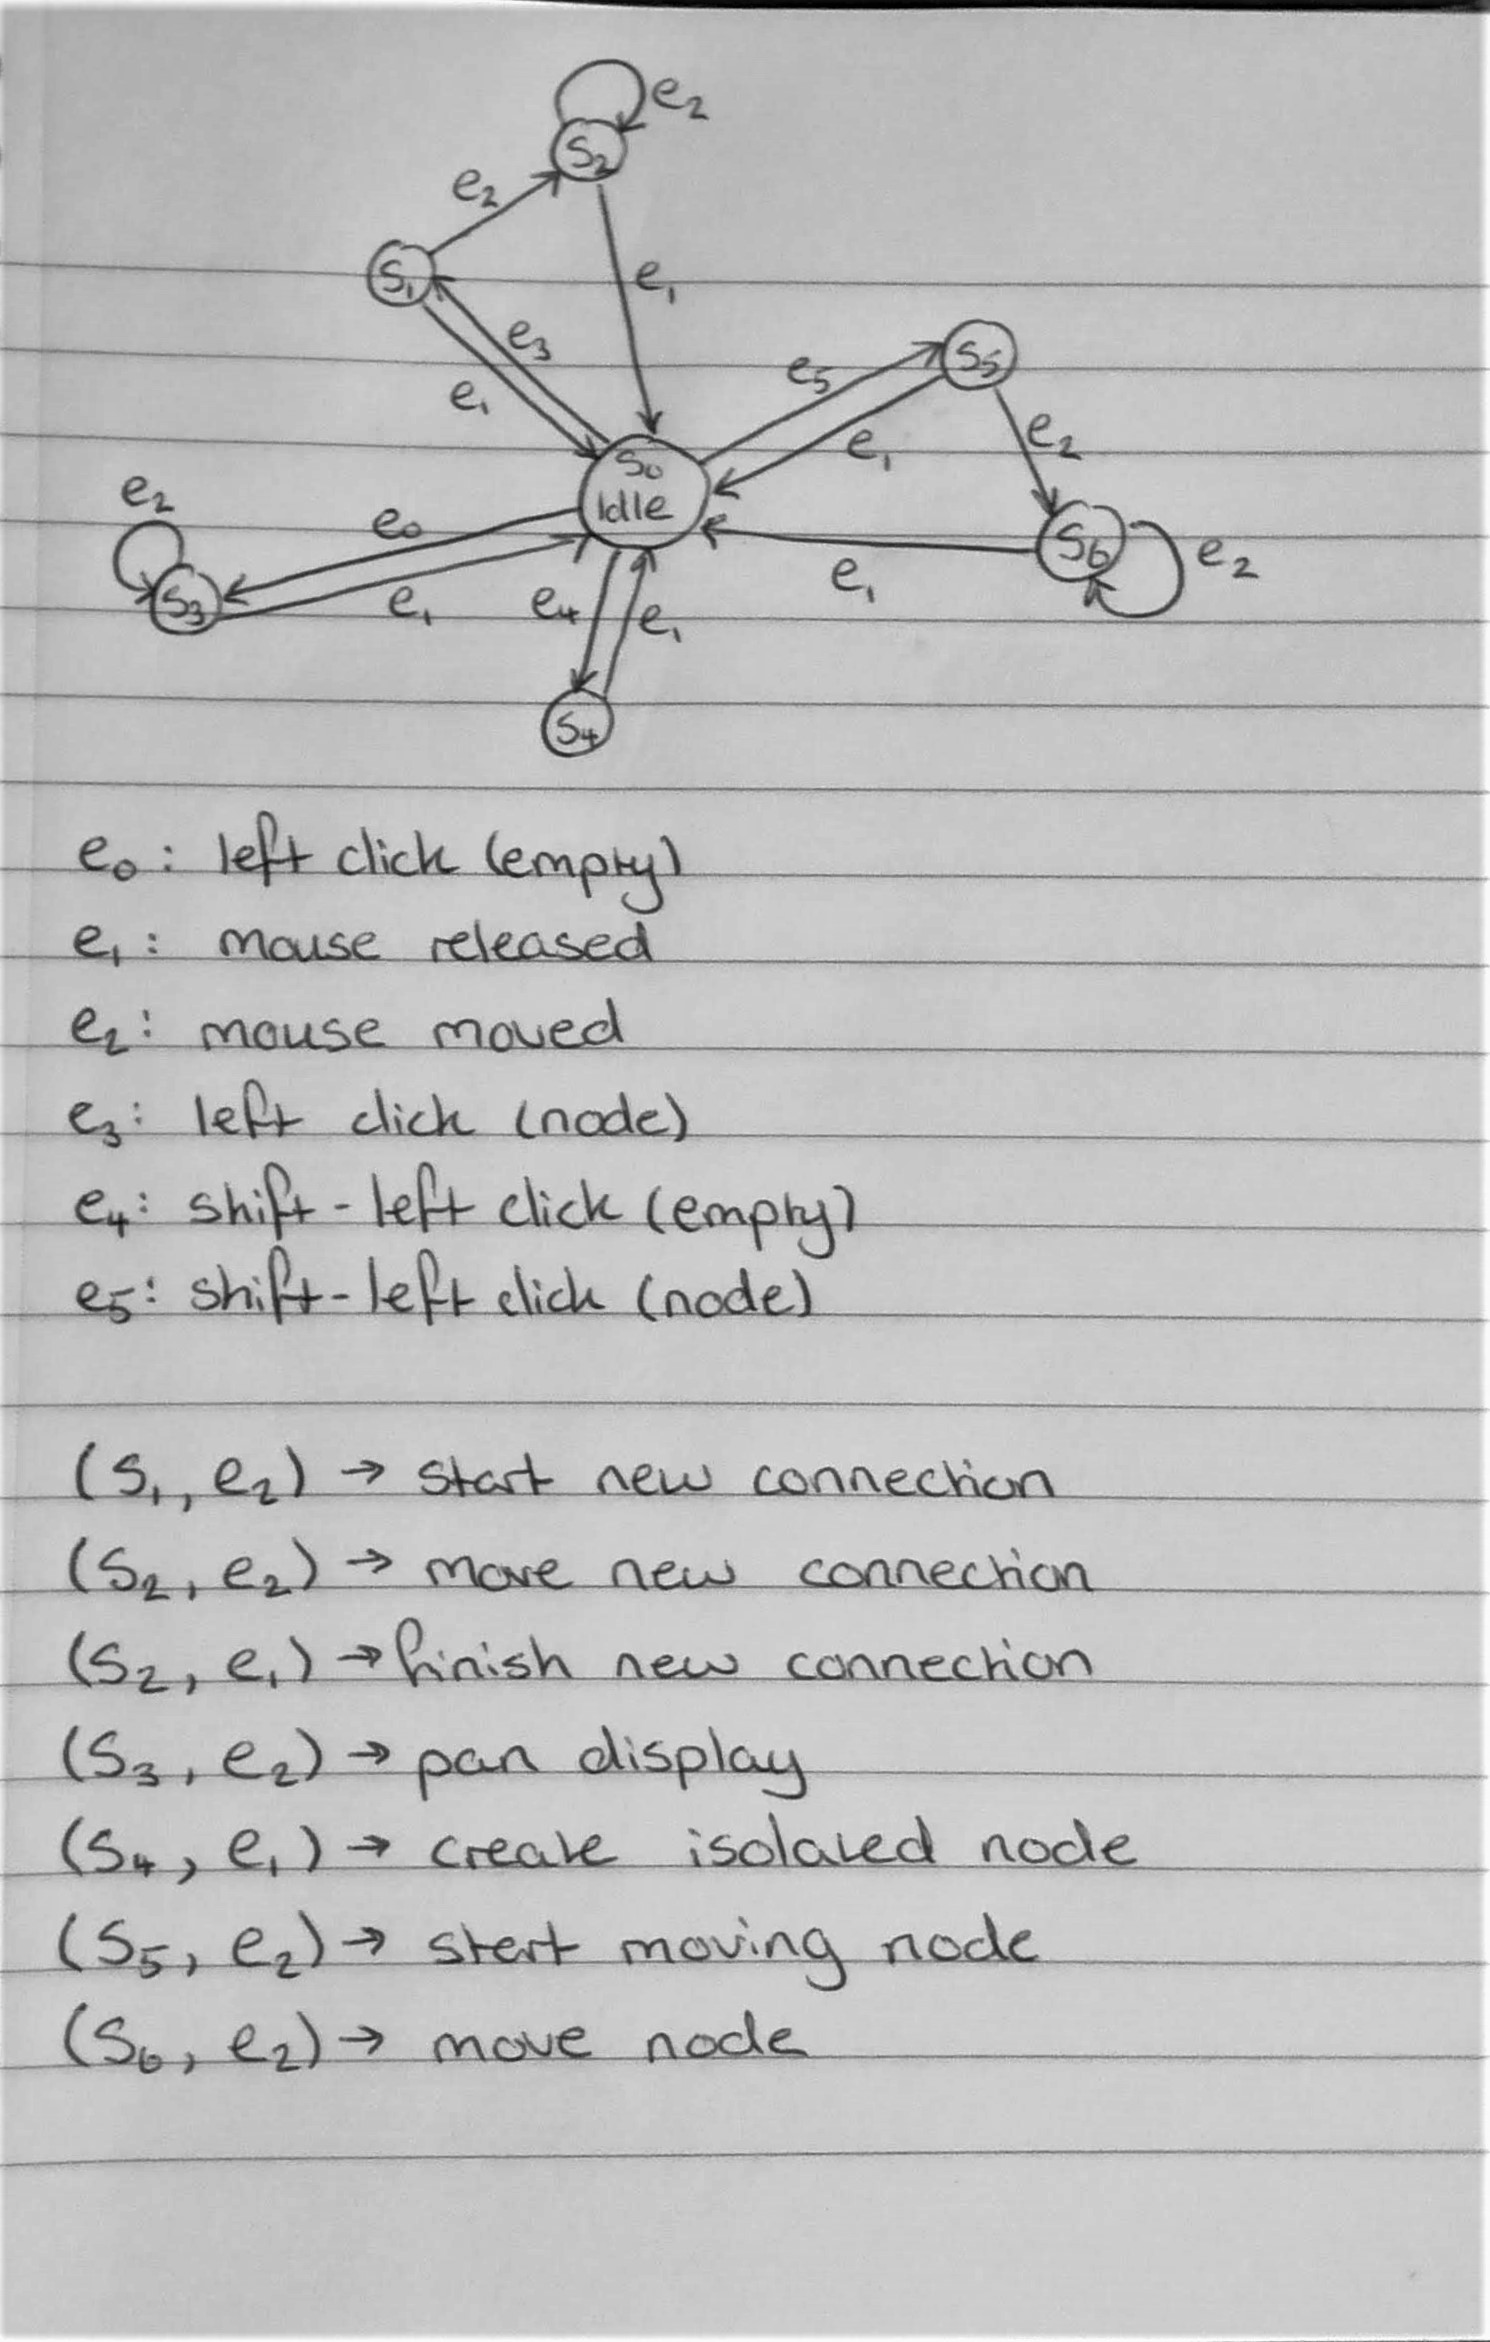
\includegraphics[width=0.5\textwidth]{network-builder-state-machine.jpg}
                \caption{Details of the network builder controls state machine}
                \label{network-builder-state-machine}
            \end{figure}

        \subsubsection{Undo/Redo Procedures}
            This program will include undo/redo functionality on the network construction component specifically, this will be modelled using two stacks, one containing the user actions that have occurred (the previous states stack) and the other containing the actions that have been reapplied from the previous states stack (the future states stack). \autoref{undo-redo-diagram} shows a diagram of the undo-redo procedures, popping from one stack and pushing into the other.

            \begin{figure}
                \centering
                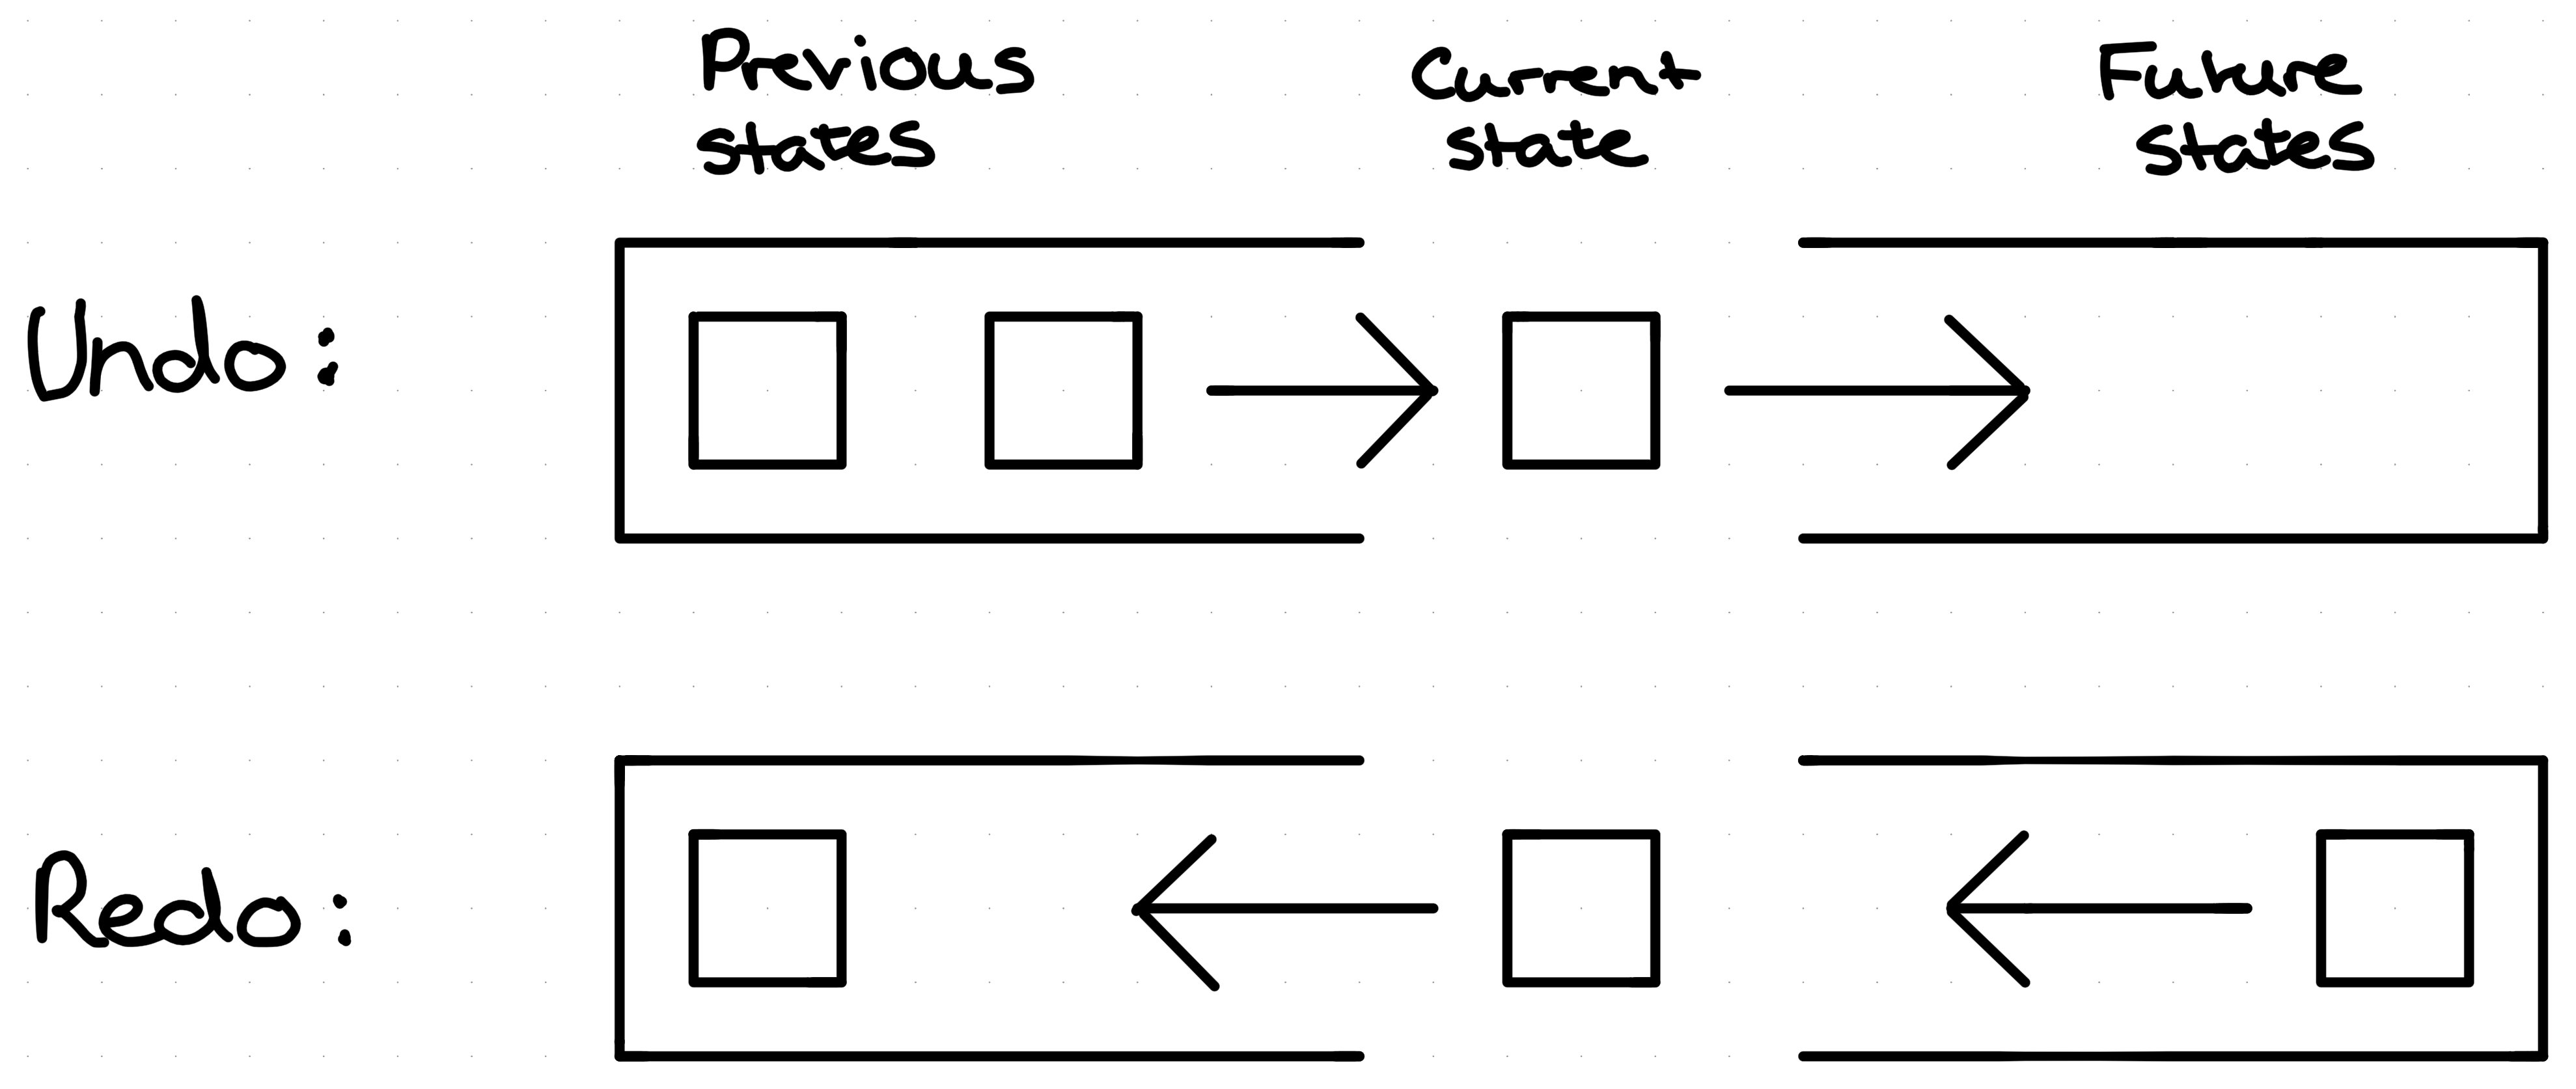
\includegraphics[width=0.9\textwidth]{undo-redo-diagram.jpg}
                \caption{Diagram showing the undo-redo procedures}
                \label{undo-redo-diagram}
            \end{figure}

    \subsection{Road geometry}

    The roads will be modelled using a series of Bezier curves, to allow for this the user must be able to adjust the control points of the curves. The edges of the graph will need to store a data structure containing 2 control points for the curve (the first and last points are defined by the source and destination nodes of the edge). This will make for cubic Bezier curves which will be controlled by their own \mintTS{CubicBezier} class. One function of this will be a \mintTS{get_point_at_distance} method which will interpolate linearly along the length of the curve, returning a point. This is not a trivial problem and my solution is documented below.

    \paragraph{Linear interpolation of cubic Bezier curves}

    Given a cubic Bezier curve with control points $\mathbf{P_0}$, $\mathbf{P_1}$, $\mathbf{P_2}$ and $\mathbf{P_3}$. We can define it as

    \[B(t) = (1 - t)^3\mathbf{P_0} + 3(1 - t)^2t\mathbf{P_1} + 3(1 - t)t^2\mathbf{P_2} + t^3\mathbf{P_3} : 0 \leq t \leq 1\]

    The $t$ parameter does not interpolate linearly across the curve. The distances between successive points is not constant. This is an issue as cars will need to move at a given speed along these curves.

    In order to fix this problem I will need to compute a point along the curve at a specific distance. My proposed algorithm consists of two steps:

    First, generate a map containing a series of length samples along the curve. This algorithm will approximate the curve as a series of small line segments and as the distance between sample points gets smaller, this approximation will improve. The pseudocode for this is shown in Algorithm \ref{generate-lookup-algorithm}

    Secondly, to get a point at a specific distance along the curve, iterate over the map to find the first value of $t$ such that $\text{map}(t) \geq \text{targetDistance}$. This algorithm is documented in Algorithm \ref{get-point-at-distance-algorithm}

    \begin{algorithm}
        \begin{algorithmic}
            \State distance $\gets 0$
            \State $t \gets 0$
            \While{$t <= 1$}
                \State \Call{map.set}{$t$, distance}
                \State $p \gets$ \Call{interpolate}{$t$}
                \State $t \gets t + \text{interpolationResolution}$
                \State $q \gets$ \Call{interpolate}{$t$}
                \State distance $\gets$ distance $+ \sqrt{(p_x - q_x)^2 + (p_y - q_y)^2}$
            \EndWhile{}
            \State \textbf{return} map
        \end{algorithmic}
        \caption{Generating a distance lookup table for a Bezier curve}
        \label{generate-lookup-algorithm}
    \end{algorithm}

    \begin{algorithm}
        \begin{algorithmic}
            \Function{get\_point}{B, targetDistance}
                \For{$t$, distance \textbf{in} B.map}
                    \If{distance $\geq$ targetDistance}
                        \State \textbf{return} $t$
                    \EndIf
                \EndFor
                \State \textbf{return} 1
            \EndFunction
        \end{algorithmic}
        \caption{Finding the $t$-value for a point at a specific distance along the curve}
        \label{get-point-at-distance-algorithm}
    \end{algorithm}

    Using these algorithms I generated \autoref{bezier-interpolation-comparison-graph} and \autoref{bezier-interpolation-comparison-on-curves}. \autoref{bezier-interpolation-comparison-graph} shows an extreme case with a relatively high value for the $\textbf{interpolationResolution}$ constant, however it is clear that this approximates the curve relatively well.

    \begin{figure}
        \centering
        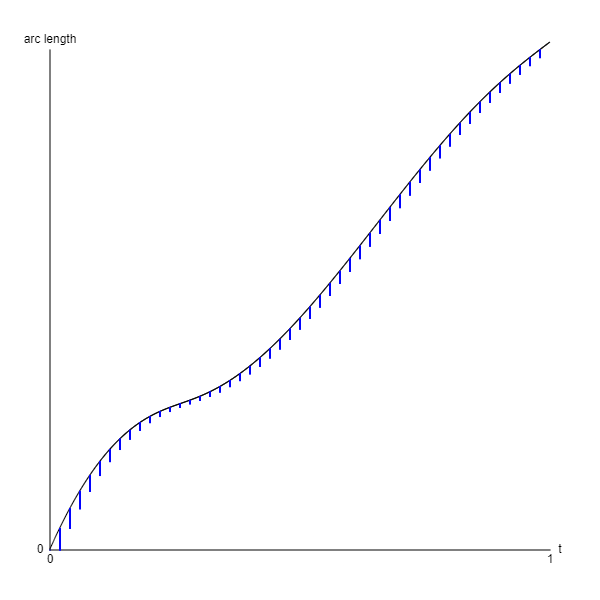
\includegraphics[width=0.6\textwidth]{LUT_bezier_interpolation.png}
        \caption{Plot showing the lookup table approximation (blue) for points at a given distance}
        \label{bezier-interpolation-comparison-graph}
    \end{figure}

    \begin{figure}
        \centering
        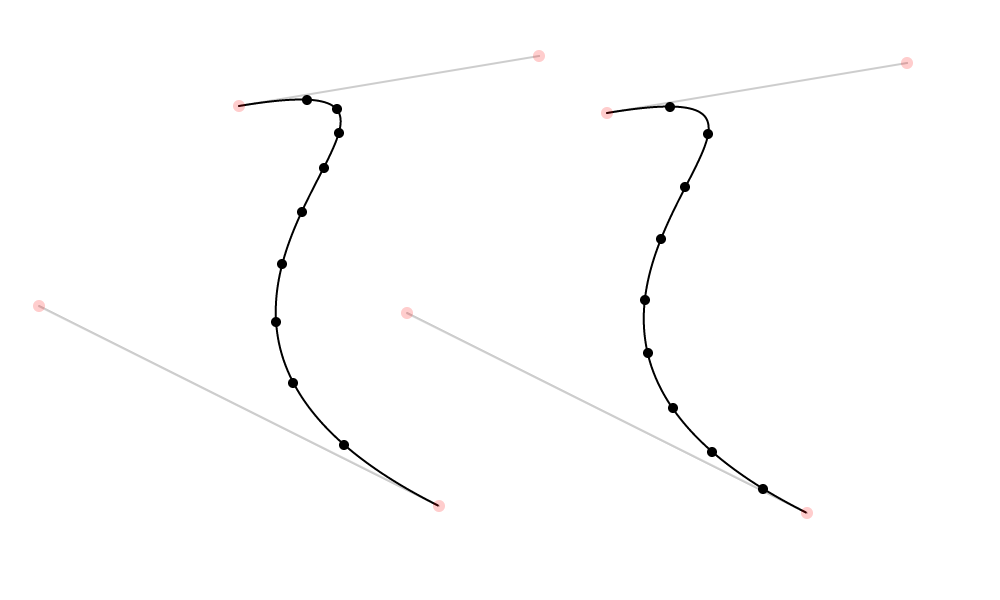
\includegraphics[width=0.6\textwidth]{bezier-interpolation-comparison.png}
        \caption{Points on the left diagram are spaced evenly by $t$-value, while ones on the right are spaced evenly by distance using the previous algorithms}
        \label{bezier-interpolation-comparison-on-curves}
    \end{figure}

    \subsection{GUI}

\section{Class structure}

    \begin{figure}
        \centering
        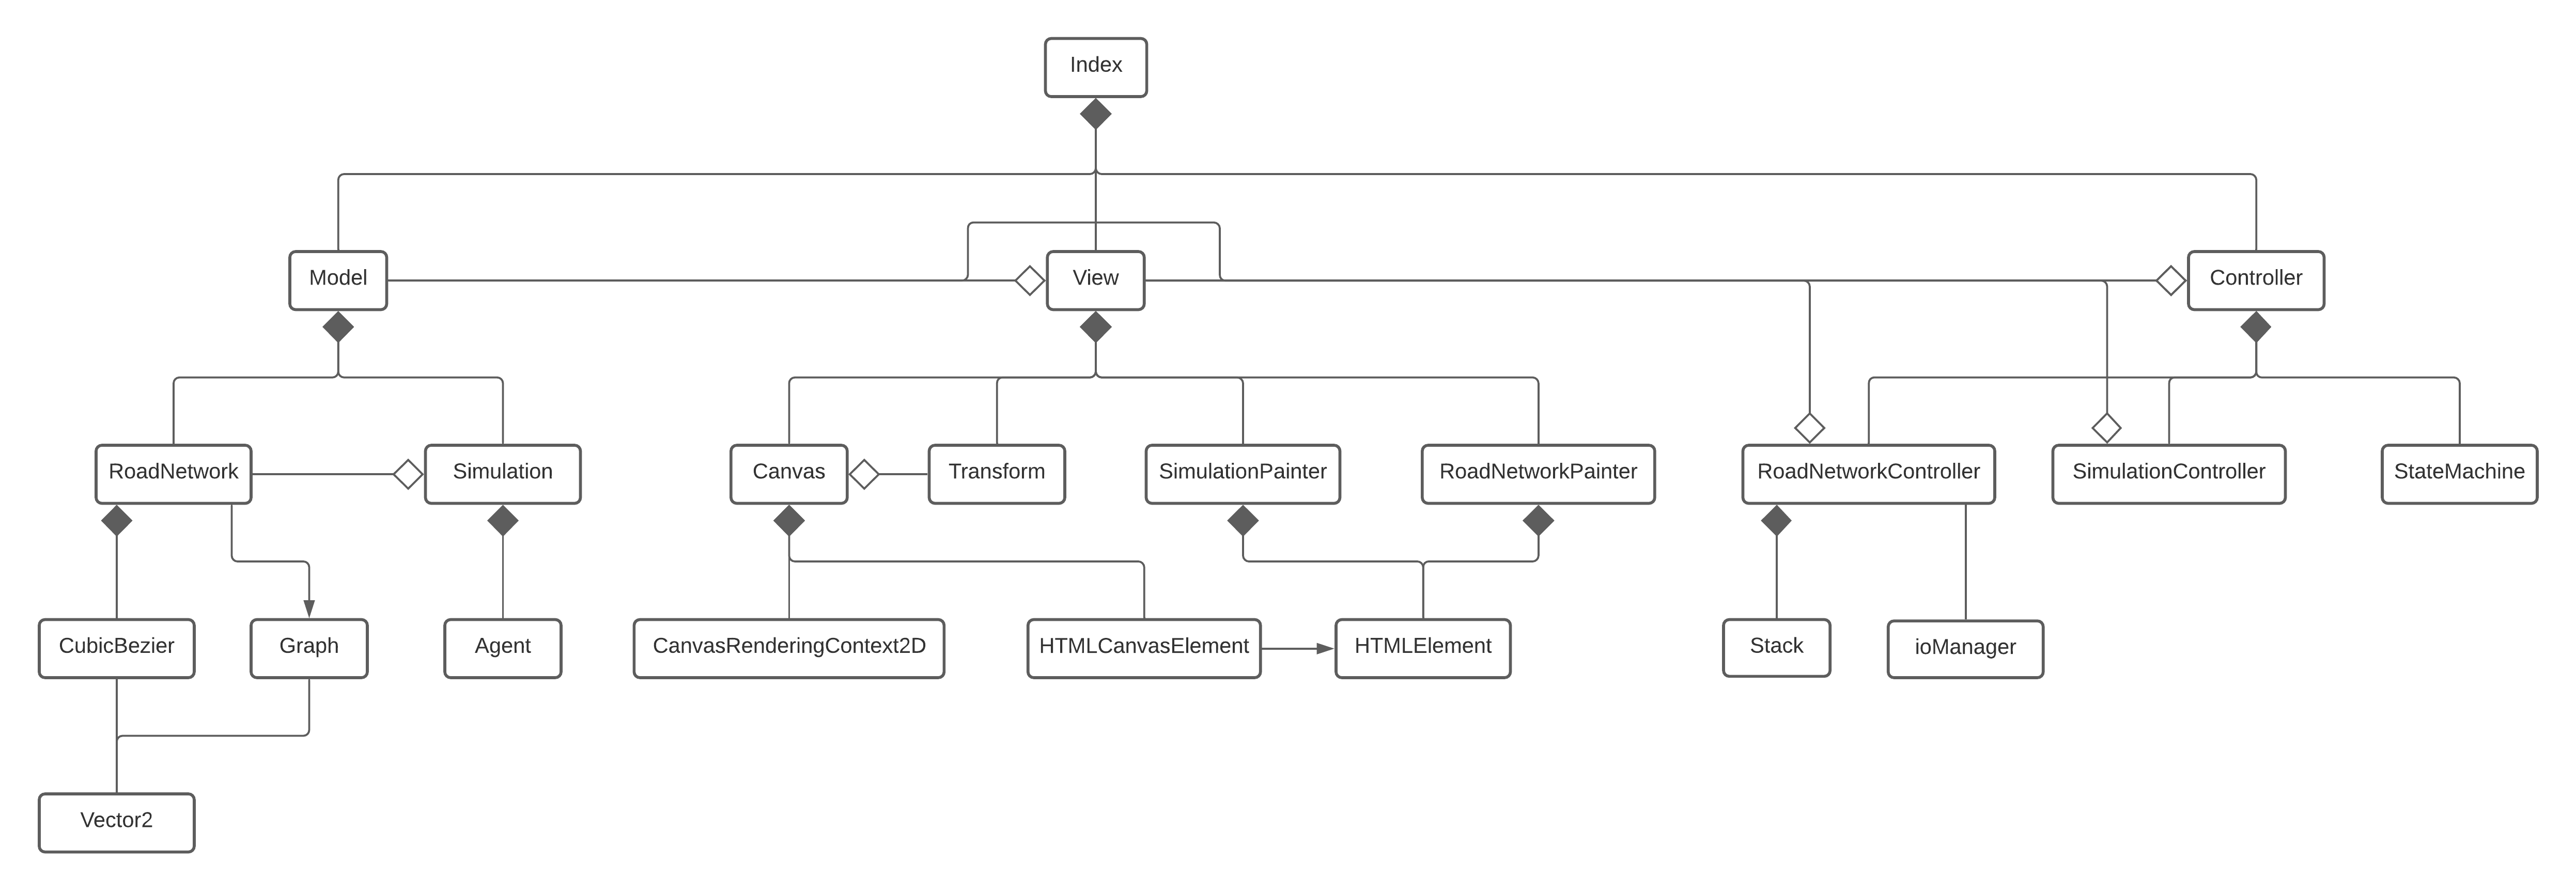
\includegraphics[angle=90,width=0.48\textwidth]{class_diagram_overview.png}
        \caption{Program class diagram}
        \label{complete-class-diagram}
    \end{figure}

    % REFACTOR THIS ################################################################
    \autoref{complete-class-diagram} shows a complete class diagram for the program, specific class relations may change during development but the main structure should remain constant, this program uses a mix of composition, aggregation and inheritance

    % \paragraph{Vector2 -}
    %
    %     This program is based in a 2D rendering environment so a general 2D Vector class will be required for many functions. This class will store an x and y numerical attribute as well as containing the following static methods:
    %
    %     \mintTS{Vector2.add(a, b)},
    %     \mintTS{Vector2.sub(a, b)},
    %     \mintTS{Vector2.mult(v, x)},
    %     \mintTS{Vector2.mag(v)},\\
    %     \mintTS{Vector2.sqr_mag(v)},
    %     \mintTS{Vector2.dot(a, b)}
    %
    %     And their non-static counterparts:
    %
    %     \mintTS{v.add(b)},
    %     \mintTS{v.sub(b)},
    %     \mintTS{v.mult(x)},
    %     \mintTS{v.mag()},
    %     \mintTS{v.sqr_mag()},
    %     \mintTS{v.dot(b)}
    %
    %     Each of these methods will be implemented with static and non-static variants, allowing for more flexible usages. I will be using methods that do not mutate their parameters which is a scheme I am more familiar with and allows for clearer syntax.
    %
    %     \paragraph{CubicBezier -}
    %
    %     This class will store all of the computation needed to model cubic Bezier curves which I explored in \autoref{bezier}.
    %     This class will contain the following methods:
    %
    %     \mintTS{b.get_vertex(i)},
    %     \mintTS{b.set_vertex(i, v)},
    %     \mintTS{b.generate_lookup()},
    %     \mintTS{b.interpolate(t)}, \\
    %     \mintTS{b.tangent(t)},
    %     \mintTS{b.second_derivative(t)},
    %     \mintTS{b.curvature(t)},
    %     \mintTS{b.get_t_at_distance(d)}, \\
    %     \mintTS{b.get_point_at_distance(d)},
    %     \mintTS{b.get_tangent_at_distance(d)},
    %     \mintTS{b.get_curvature_at_distance(d)}
    %
    %     \paragraph{State Machine -}
    %
    %     This class represents a finite state machine model which utilises function callbacks, it will store a list of transitions and callbacks. When the \mintTS{transition} method is called the state will change based on the appropriate transition and the callback assigned to it will be executed.
    %
    %     The included methods are:
    %
    %     \mintTS{sm.transition(e)}, \mintTS{sm.add_rule(src, e, dst, cb)}
    %
    %     \paragraph{Stack -}
    %
    %     I will also include a stack implementation to be used in the undo/redo procedures. Including:
    %
    %     \mintTS{s.push(e)}, \mintTS{s.pop()}, \mintTS{s.is_empty()}, \mintTS{s.clear()}

\section{Model}

    The model component is responsible for encapsulating the modelling data structures of the program. In this case the model is a graph structure containing road network information as well as a simulation containing a series of agents present in the network.

    \subsection{Classes}

        \subsubsection{Model}

            The Model class is the container for all other classes in this component. Containing methods for the view and controller components to interact with it. It will encapsulate the RoadNetwork and Simulation classes. The Model class also contains a series of methods used by the controller class during transition callbacks.

            \umldiagram{Model}{
                \mintTS{- roadNetwork: RoadNetwork}\\
                \mintTS{- roadNetwork: RoadNetwork}\\
                \mintTS{- simulation: Simulation}
            }{
                \mintTS{+ copy_road_network(): RoadNetwork}
            }

        \subsubsection{RoadNetwork}

            The RoadNetwork class represents the data structure for the road network, inheriting from the Graph class and implementing its generic types.

            \umldiagram{RoadNetwork}{}{
                \mintTS{+ get_bezier(number, number): CubicBezier}\\
                \mintTS{- get_edge_length(number, number): number}\\
                \mintTS{+ find_route(number, number): number}
            }

        \subsubsection{Simulation}

            The Simulation class is responsible for managing a series of agents that traverse the road network.

            \umldiagram{Simulation}{
                \mintTS{- roadNetwork: RoadNetwork}\\
                \mintTS{- agents: Agent[]}\\
                \mintTS{- sources: number[]}\\
                \mintTS{- exits: number[]}
            }{
                \mintTS{+ step(): void}\\
                \mintTS{- add_agent(number, number): void}\\
                \mintTS{+ agent_count(): number}\\
                \mintTS{- find_terminating_vertices()}\\
                \mintTS{+ get_agent_position(number): Vector2}\\
                \mintTS{+ get_agent_rotation(number): number}\\
                \mintTS{- get_agent_bezier(number): CubicBezier}
            }


        \subsubsection{CubicBezier}

            This is the container for the geometric structure of a cubic Bezier curve, outlined in \autoref{bezier}. Containing methods for querying and operating on these curves.

            \umldiagram{CubicBezier}{
                \mintTS{- vertices: Vector2[]}\\
                \mintTS{- distanceLookup: Map<number, number>}
            }{
                \mintTS{+ get_vertex(number): Vector2}\\
                \mintTS{+ set_vertex(number, Vector2): void}\\
                \mintTS{- interpolate(number): Vector2}\\
                \mintTS{- tangent(number): Vector2}\\
                \mintTS{- second_derivative(number): Vector2}\\
                \mintTS{- curvature(number): number}\\
                \mintTS{- generate_lookup(): void}\\
                \mintTS{+ get_t_at_distance(number): number}\\
                \mintTS{+ get_point_at_distance(number): Vector2}\\
                \mintTS{+ get_tangent_at_distance(number): Vector2}\\
                \mintTS{+ get_curvature_at_distance(number): number}
            }

        \subsubsection{Graph}

        After exploring the different types of graph structure I have decided to utilise the adjacency matrix structure for this project. Despite the adjacency matrix implementation having less scalable complexities for most functions [\autoref{graph-time-complexities}] it has a large benefit of a constant time edge lookup; since this function will be called many times for each agent in the network I anticipate this implementation will be more efficient in the long term.

        \umldiagram{Graph}{
            \mintTS{- adjacencyMatrix: Edge[][]}\\
            \mintTS{- vertices: Vertex[]}
        }{
            \mintTS{+ size(): number}\\
            \mintTS{+ add_vertex(Vertex): number}\\
            \mintTS{+ set_vertex(number, Vertex): void}\\
            \mintTS{+ get_vertex(number): Vertex}\\
            \mintTS{+ remove_vertex(number): Vertex}\\
            \mintTS{+ set_edge(number, number, Edge): void}\\
            \mintTS{+ get_edge(number, number): Edge}\\
            \mintTS{+ remove_edge(number, number): Edge}
        }

\section{Network Testing}

    \subsection{Traffic Behaviour Modelling}

    In this simplified model the only variable the 'drivers' have access to is the acceleration of the vehicle. This parameter will be governed by a series of specific rules listed below:

    \begin{itemize}
        \item Agents will slow when a car in it's direction of travel is too close. Attempting to maintain a good separation distance from the Agent in front.

        \item Agents will attempt to maintain a speed proportional to the curvature of the road, travelling at reduced speeds along tighter bends.

        \item When the road is clear and straight Agents will accelerate up to some reasonable maximum speed.

        \item Agents will attempt to maintain a similar speed to the other Agents closest to them.
    \end{itemize}

    \subsection{Agent Structure}

    In order to simulate real-world traffic the 'cars' (here out referred to as Agents) will need to encapsulate the following information:

    \begin{itemize}
        \item Speed - This will be used to update the Agent's position
        \item Position - This will be a proportionate value representing the distance travelled along it's current edge
        \item Route - This will be generated using a path finding algorithm and determines the direction the Agent will choose to go at a junction
    \end{itemize}

    \subsection{Maximum Graph Flow}

    \subsection{GUI}

    \subsection{Bezier Curvature}
